\chapter{Results}
This chapter discusses the results of our project. A description of the built application will be given, alongside with screenshots.
Also, graphs will be used to show the performance of our application.

\section{SwiftTV}
Since we built a download and stream application for the Samsung SmartTV based on libswift, we dubbed our application SwiftTV.
The name is kept simple because other existing applications based on libswift have similar names. This section explains how SwiftTV works.
\\\\
// Screenshot of main menu here 
\\\\
The main menu points to the four different pages in the application, browse, downloads, player and settings. When selecting one of these pages the main menu remains visible.
\\\\
// Screenshot of browse here 
\\\\
Browse is where you can either browse your local filesystem to play a media file or search the internet for files to download or stream. Browsing the local filesystem is done with features included in the Samsung API and is therefor all done in JavaScript. When choosing a file from the browser it can be added to the playlist in the player page to be played. The search functionality sends a "/search:searchTerm" request to the HTTP server which in turn starts a search using Dispersy. After some time the search results are requested by JavaScript using a "/results" request. The results are returned in the form of an XML file and shown on screen. 
\\\\
The user can select one of these results and choose to either download ot stream it. JavaScript either sends a "/add:hash" or "/stream:hash request" depending on the choice. If download is chosen the the download is added to the list in DownloadManager and start downloading. If stream is chosen a stream is opened and is added to the playlist on the player page.
\\\\
// Screenshot of player here 
\\\\
Player is where videos and streams can be viewed. To view videos or streams they must first be added to the playlist while in the browser. Videos will start playing in the small screen but full screen can be enabled afterwards.
\\\\
// Screenshot of downloads here 
\\\\
Downloads is where the current list of downloads can be viewed. Downloads can be paused, stopped and resumed. JavasScript will send "/pause:hash", "/remove:hash" and "/resume:hash" requests to do this. When stopping a download it will be removed from the list. 
\\\\
// Screenshot of settings here 
\\\\
In the settings page users can set their maximum download and upload speed as well as the download location. These settings are saved in memory and loaded on startup. When the settings are changed JavaScript sends a "/settings:upspeed:downspeed:downloadpath" request to the HTTP server.


\section{Measurements}
For this section, we measured the CPU and memory usage of the application. We measured these values against time and the download speed.

\newpage
\subsection{Memory/CPU usage while idle}

\begin{center}
\begin{figure}[h]
	\centering
	\mbox{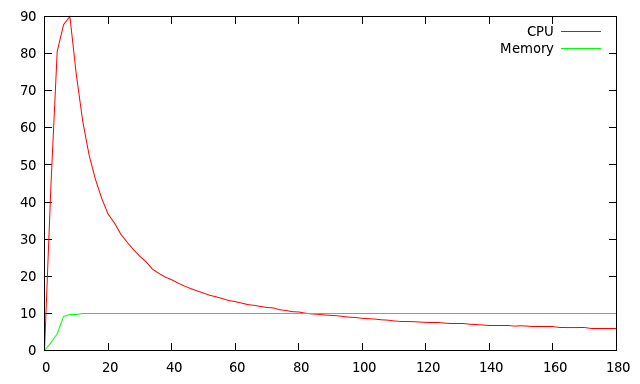
\includegraphics[width=1.2\textwidth]{Images/idle.png}}
	\label{graph:idle}
	\caption{CPU and memory usage while the TV is only running the application, not doing anything else.}
\end{figure}
\end{center}
